\documentclass[11pt]{article}
\usepackage{amsmath}
\usepackage{amsfonts}
\usepackage{graphicx}
\usepackage[margin=0.5in]{geometry}
\newcommand{\Z}{\mathbb{Z}}
\usepackage{hyperref}
\usepackage{subcaption}
\author{Peter Lee}
\date{\today}
\title{Examination of Gated Recurrent Networks for Forecasting the Mackey-Glass Time series}

\begin{document}
\maketitle

\section{Introduction}
A common application of recurrent neural network (RNN) models is the
analysis patterns within time series. A specific
type of analysis is predictive forecasting, where one uses past
observations to predict those in the future. 

The Mackey-Glass (MG) series \cite{MG} is known as a chaotic time series.
The MG series's chaotic behaviour, when its parameters and initial
conditions enable it to undergo bifurcation, makes it interesting
for predictive forecasting, since it does not have a general
solution. In the literature there has been many attempts of using deep
learning models to forecast the MG
series. Lanedes \textit{et al.} used a multi-layer perceptron with past control
points to calculate a non-linear approximation for forecasting future
points \cite{tr}. Farsa \textit{et al.} used the same configuration as
\cite{tr} and through the comparison of their NARX-Elman network they showed
that there are many works that use the MG series as a way to validate
their time series regression models \cite{Farsa}.

In this paper I will be investigating whether gated recurrent networks
perform better than other non-gated recurrent and non-recurrent models for predictive
forecasting. More specifically, I will be investigating two types of
gated recurrent networks, Long Short Term Memory (LSTM) \cite{LSTM}
and Gated Recurrent Units (GRU) \cite{GRU} and comparing them to the Elman (ELM) recurrent neural network and a Multi-Layer Perceptron (MLP) model. The MLP was constructed in a similar style to the one used by \cite{tr}. The hypothesis for these experiments was that the gated recurrent models would outperform the non-gated models.

Two experiments were conducted for forecasting future MG values 1, 5,
10, and 30 steps ahead. The first is when the models fit to the same MG series with static parameters as \cite{tr,Farsa}. The second experiment fit models to MG series with
a free parameter to evaluate if the models could adapt to the shape of
the curve during evaluation. 

%REDO
The first experiment showed that the gated RNNs held no consistent improvement in prediction over
the other models within the number of network structures attempted. Evaluations of distant predictions increased
error for each model, but did not provide any evidence that gated RNNs were superior. The second experiment showed that the MLP was unable to generalize to
having a randomized parameter. However, the performance between all the
recurrent networks remained similar. Although predicting distant
values increased error rates much more than the first experiment,
there was still little notable difference between the recurrent
models.

These predictive forecasting experiments showed that there was
little tangible benefit from using a gated network instead of an
ordinary Elman network. This suggests that
the gated network's structure to forget information may be
better suited for tasks that require active recall, like NLP tasks, instead of ones like
predictive forecasting that can be acquired by analyzing continous steps.

\section{Models}
The MLP is a model that uses hidden layers of non-linear functions, as shown in equation (\ref{eq:MLP_h}),
to approximate a target function. RNNs are MLPs that use previous evaluations
of hidden nodes as input, forming recurrent connections. A simple example of an RNN is the Elman network, with hidden nodes calculated in
equation (\ref{eq:RNN_h}).
Gated recurrent networks are networks that control the
amount of information that is held in hidden nodes between time
steps. With these gates, the model can selectively ``forget''
and ``focus'' on information. It is thought that their ability to select what information
passes to subsequent time steps is what enables them to perform so
well in various tasks \cite{LSTM}. The LSTM was introduced in the early
1997, while the GRU was introduced in 2014 \cite{GRU}. It has been theorized
that the GRU is able to perform equally as well as the LSTM in many tasks \cite{Chung}, with the benefit of having reduced parametric complexity. 
The hidden nodes for
LSTM and GRU are calculated by equations (\ref{eq:LSTM_h}) and (\ref{eq:GRU_h})
respectively. \footnote{Implementation code can be found at \url{https://github.com/PeterQLee/CSCI4192}}
%Split up??
\begin{equation}
\mathbf{h} = f( W_xx+B)
\label{eq:MLP_h}
\end{equation}
\begin{equation}
\mathbf{h^t} = \tanh(W_xx+W_hh^{t-1}+B)
\label{eq:RNN_h}
\end{equation}
%Fill in equations
\begin{equation}
\begin{split}
f^{t} = \sigma(W_{xf}x + W_{hf}h^{t-1}+B_f) \\
i^{t} = \sigma(W_{xi}x + W_{hi}h^{t-1}+B_i) \\
`c^{t} = \tanh(W_{xc}x+W_{hc}h^{t-1}+B_c) \\
c^{t} = c^{t-1} \circ f^{t} + i^{t} \circ `c^{t} \\
o^{t}= \tanh (W_{xo}x + W_{ho}h^{t-1} + B_o) \\
h^{t} = o^{t} \circ c^{t}  \\
\end{split}
   \label{eq:LSTM_h}
\end{equation}
\begin{equation}
\begin{split}
  z^{t} = \sigma(W_{xz}x + W_{sz}s^{t-1} + B_z) \\
  r^{t} = \sigma(W_{xr}x + W_{sr}s^{t-1} + B_r) \\
  h{t} = \tanh(W_{xh}x + W_{sh}s^{t-1} + B_h) \\
  s^{t} = (1-z) \circ h^{t} + z \circ s^{t-1} 
\end{split}
\label{eq:GRU_h}
\end{equation}
\begin{center}$\sigma$: sigmoid function\\$f$: nonlinear function\\$\circ$ Hadamard product\end{center}
All these models were implemented in Tensorflow. Batch sizes of 1 were
used and AdamOptimizer \cite{adam} was used to train with a learning rate set at $10^{-3}$. For predictive forecasting, the recurrent networks
were trained by predicting an entire future sequence with back propagation through
time. The MLP was trained by predicting future values using four
control points, $x(t), x(t-6), x(t-12), x(t-18)$ with back propagation, similar to \cite{tr}.

\section {Methods}
\subsection {Mackey-Glass Time Series}
MG series is modelled by the differential equation (\ref{eq:MG}).
\begin{equation}
  \begin{split}
\frac{dx(t)}{dt} = \frac{\beta x(t-\tau)}{1+x^n(t- \tau)} - \gamma x(t); \tau,\beta,n,\gamma > 0.
\label{eq:MG}
  \end{split}
\end{equation}
To generate the MG series, I used a 4 point Runge-Kutta (RK4) method to
integrate the differential equation, with a step size of
0.01 and range of $0 \leq t \leq 1000$. This implementation was created in Python, using a queue
data-structure to recall the recurrent values. For training, only
$0 \leq t \leq 500$ were used and similarly for testing 
$500 < t \leq 1000$  were used, with the restriction $t \in \Z$. The data vectors used
for input and labels were $X = x(t) $ and $ Y = x(t+t_0) \forall
t$, given some delay $t_0$. 

The forecasting task involves predicting $x(t+t_0)$, given previous
information $x(t), x(t-1), ..., x(1)$. In general models for predictive forecasting
attempt to estimate $x(t+t_0)$, as shown in equation
(\ref{eq:pred_forecast}) The goal of training is to 
choose parameters, $\theta$, to minimize the error between $x(t+t_0)$
and $f$. In this case, I used mean squared error as the error function.
\begin{equation}
  x(t+t_0) \approx p(x(1);x(2);x(3)...x(t) | \theta)
  \label{eq:pred_forecast}
\end{equation}

\subsection{Experiments}
For each of the following
experiments, I
trained models with two layers of hidden nodes with sizes of 32, 64, 96, and 128 to
view the models with range of different hyper parameters and observe if
there was a trend in performance with increased complexity. For each
initialization I attempted forecasting with $t_0$ = 1, 5, 10, and 30,
to determine the degredation of performance with further forecasting.

%\subsection {Experiment 1: Constant MG Parameters}
The first experiment followed those of related works \cite{tr, Farsa},
by having the
parameters of the MG series kept constant to $\beta = 0.2$,
$\gamma = 0.1$, $\tau = 17$, and $n = 10$ and $x(t)=1.2  \forall  t \leq 0$. These models were tested 10 times for each configuration, using Xavier initialized variables \cite{Xavier}. The second experiment used 10 MG series with different
initializations of $0.1 \leq \beta < 4$ and the remaining MG parameters the same as experiment 1. A leave-one-out style evaluation was employed by using 9 different series as a training
set, while the last one was used as a training set. The motivation of
this experiment, which contrasts those of other authors, was to measure
how well the recurrent models could adapt to the shape of the curve during
evaluation by essentially estimating the randomized parameter.

\subsection{Evaluation}
\label{sec-3-3}
To measure model performance, two metrics were selected. They are
the cumulative absolute difference (\ref{eq:cumabs}) and the
cumulative absolute difference of slopes
(\ref{eq:cumabsderiv}). The cumulative absolute difference, which is
equivalent to square root mean squared error, is used 
in \cite{Farsa}, and generally shows how far off each prediction
is from the truth. The cumulative absolute difference of slopes is
unique to this paper, and its purpose is to show whether a model can
adapt to sharp peaks in the functions, or whether the model just
generalizes to a smooth approximation of the curve. Values of these metrics that are closer to 0 indicate better performance.

%Xavier initialization
\begin{equation}
  \int_{t_{start}}^{t_{end}} | x(t) - p(t) |
\label{eq:cumabs}
\end{equation}
\begin{equation}
  \int_{t_{start}}^{t_{end}} | \frac{dx(t)}{dt} - \frac{dp(t)}{dt} |
\label{eq:cumabsderiv}
\end{equation}

\section {Results}
\subsection {Experiment 1: Constant Parameters}
% Conclusions from this section
% A) LSTM and GRU do not improve performance
% B)

Within Figure \ref{fig:mg1_scatter} are the results of the
number of different configurations attempted for each forward
prediction of $t_0$. Examples of the curves that generated this data
can be found in Figure \ref{fig:func_evals} in the Appendix. Figure \ref{fig:mg1_save} condenses this information by selecting the scores for
the best performing configuration of the model in terms of
median. The GRU and LSTM do not
outperform the ELM since they never exceed the latter model outside
the iqr. The MLP also seems to be competitive with these models, with
the exception of $t_0 = 30$, where it possesses an elevated level in
both cumulative absolute difference and cumulative absolute difference
in slopes. 

% \begin{table}
%    \begin{centering}
%   \begin{tabular}{|l|l|l|l|l|}
%     \hline
%     $t_0$ & ELM & LSTM & GRU & MLP \\
%     \hline
% 1 & 0.0175 $\pm$ 0.0052 & 0.0351 $\pm$ 0.0056 & 0.0230 $\pm$ 0.0051 & 0.0396 $\pm$ 0.0365 \\
% 5 & 0.0332 $\pm$ 0.0078 & 0.0379 $\pm$ 0.0086 & 0.0535 $\pm$ 0.0195 & 0.0329 $\pm$ 0.0184 \\
% 10 & 0.0341 $\pm$ 0.0134 & 0.0415 $\pm$ 0.0091 & 0.0385 $\pm$ 0.0076 &0.0335 $\pm$ 0.0430 \\
% 30 & 0.0714 $\pm$ 0.0130 & 0.0967 $\pm$ 0.0088 & 0.0834 $\pm$ 0.0072 &0.1140 $\pm$ 0.0109 \\
%     \hline
%   \end{tabular}
%   \caption{Experiment 1: Best of median cumulative difference values for each model
%     configuration $\pm$ iqr.}
%   \label{table:cumabs1}
%   \end{centering}
% \end{table}

% %cumabs

% \begin{table}
%   \begin{centering}
%   \begin{tabular}{|l|l|l|l|l|}
%     \hline
%     $t_0$ & ELM & LSTM & GRU & MLP\\
%     \hline
% 1 & 0.0072 $\pm$ 0.0027 &0.0127 $\pm$ 0.0011 &0.0087 $\pm$ 0.0017 &0.0047 $\pm$ 0.0011 \\
% 5 & 0.0120 $\pm$ 0.0031 &0.0135 $\pm$ 0.0012 &0.0174 $\pm$ 0.0026 &0.0073 $\pm$ 0.0006 \\
% 10 & 0.0092 $\pm$ 0.0035 &0.0112 $\pm$ 0.0023 &0.0119 $\pm$ 0.0014 &0.0071 $\pm$ 0.0016 \\
% 30 & 0.0148 $\pm$ 0.0026 &0.0168 $\pm$ 0.0010 &0.0158 $\pm$ 0.0006
%                              &0.0195 $\pm$ 0.0040 \\
%     \hline
%     \end{tabular}
%     \caption{Experiment 1: Best of median cumulative difference of slopess for each
%     model configuration $\pm$ iqr.}
%     \label{table:Dcumabs1}
% \end{centering}    
% \end{table}

  % Figure \ref{fig:mg1_scatter} shows the performance of models with
  % respect to the number of parameters they possess. It can be observed
  % that all recurrent models seem to perform very similarly for $t_0 =
  % 1$. The MLP seems to fit well with less parameters, with overfitting
  % likely occuring when the number of parameters increases, as shown 
  % by the higher median and larger inter-quartile range (iqr). None of the recurrent models seem to improve or degrade with additional parametric complexity. Overall, all the models achieve similar
  % performance in fitting to the static MG series. Since the recurrent
  % models did not out perform the MLP, this raises the question as to
  % whether fitting to a static MG series is the best benchmarking task
  % for the for the series prediction models.

  \begin{figure}
    \begin{center}
      \begin{subfigure}{.48\textwidth}
        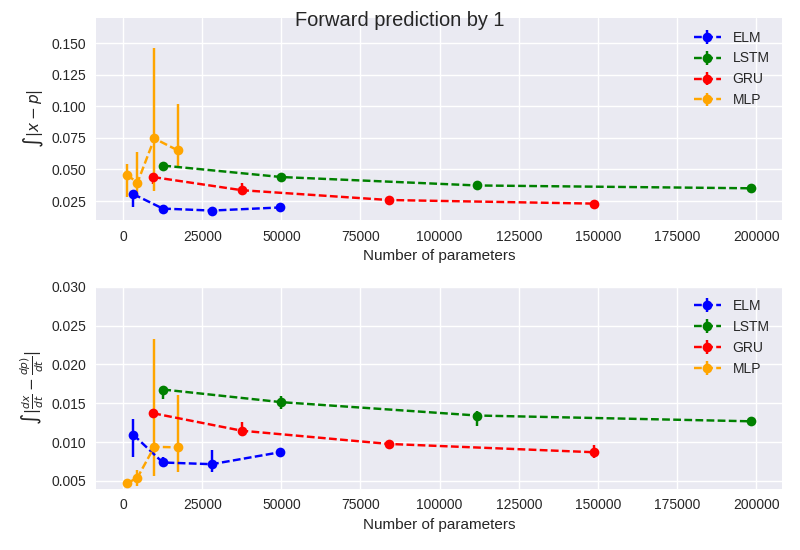
\includegraphics[width=\textwidth]{figures/mg1_scatter_1.png}
        \caption{}
      \end{subfigure}
      \begin{subfigure}{.48\textwidth}
        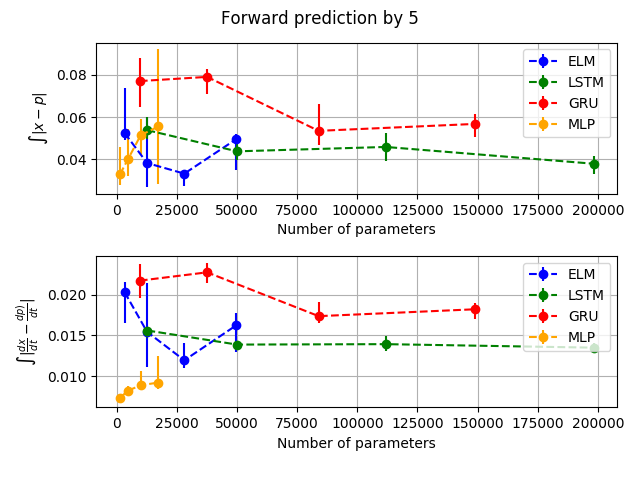
\includegraphics[width=\textwidth]{figures/mg1_scatter_5.png}
        \caption{}
      \end{subfigure}
      \begin{subfigure}{.48\textwidth}
        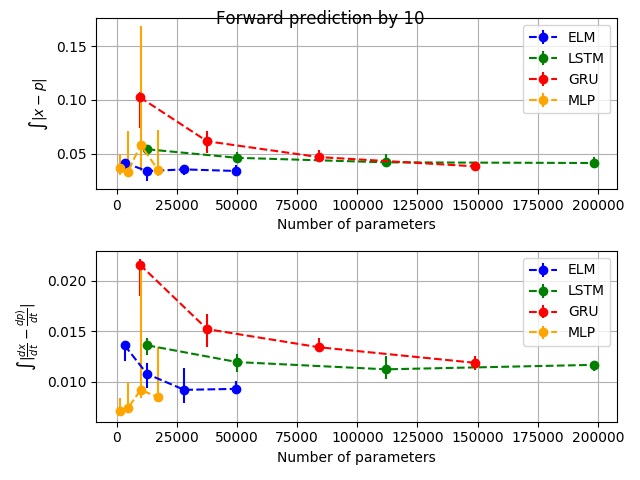
\includegraphics[width=\textwidth]{figures/mg1_scatter_10.png}
        \caption{}
      \end{subfigure}
      \begin{subfigure}{.48\textwidth}
        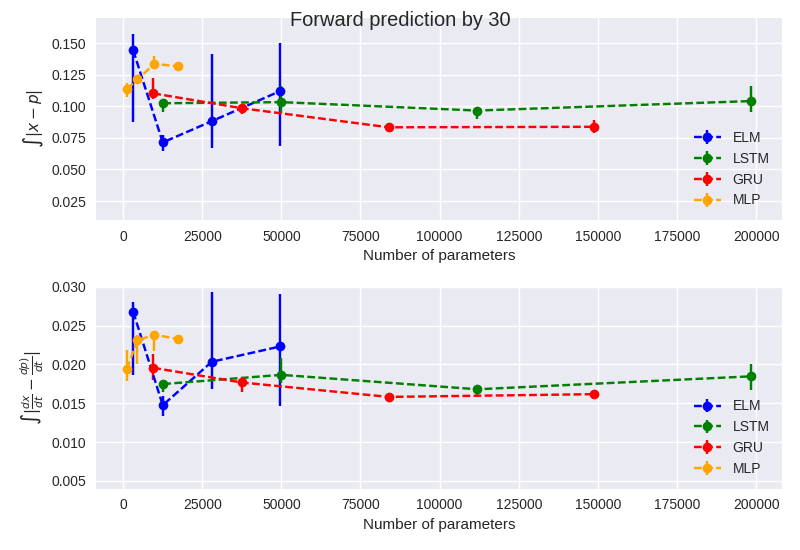
\includegraphics[width=\textwidth]{figures/mg1_scatter_30.png}
        \caption{}
      \end{subfigure}
       
    \caption{Scatter plots showing model performance with different
      network configurations in experiment 1. Using 10 evaluations with different weight
    initializations, points show the median with vertical bars
    extending 1 quartile above and below the median. The models structured with hidden node sizes of 32, 64, 96, and 128 are plotted in regards to their parametric complexity.}
    \label{fig:mg1_scatter}
    \end{center}
  \end{figure}
  
  \begin{figure}
    \begin{center}
   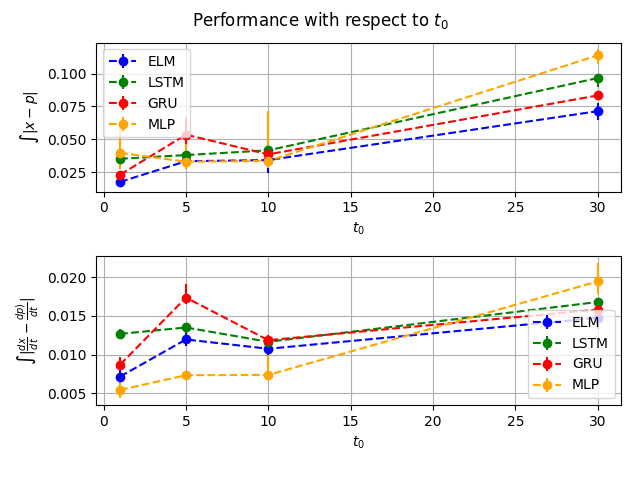
\includegraphics[width=.96\textwidth]{figures/mg1_save.png}       
    \caption{Scatter plot showing the performance trend with each forward prediction task of the ELM, GRU, LSTM, and MLP, each using the configuration (number of hidden nodes) that performed the best. Y-axis shows the performance metrics as described in section \ref{sec-3-3}.}
    \label{fig:mg1_save}
    \end{center}
  \end{figure}

  \subsection {Experiment 2: Randomized $\beta$}
  % Conclusions
  % A) Exclusion of MLP
  % B) Gated networks still don't have an advantage
  % C) Significantly degraded performance

  First, the MLP was excluded from further analysis because it became eminently clear that it
  was unable to adapt to having a free parameter (see Figure
  \ref{fig:mg2_func_MLP}).


  Similar to the first experiment,
  Figure \ref{fig:mg1_scatter} shows only marginal changes in performance with
  respect to the number of parameters they possess. Figure \ref{fig:mg2_save} once again  does not show that LSTM and GRU give better performance
  than the ELM. In contrast to experiment 1, it appears that
  the models get much more inaccurate with distant
  predictions, increasing by at least a factor of 40, compared to the factor of 3 in experiment 1. However, the performances for each model seem to
  degrade at the same rate.

%   \begin{table}[t]
%       \begin{centering}
%   \begin{tabular}{|l|l|l|l|}
%     \hline
%     $t_0$ & ELM & LSTM & GRU \\
%     \hline
%     1 & 0.1035 $\pm$ 0.0404 &0.1484 $\pm$ 0.0803 &0.1146 $\pm$ 0.0432 \\
%     5 & 0.7192 $\pm$ 0.2243 &0.7388 $\pm$ 0.1292 &0.6660 $\pm$ 0.2350 \\
%     10 & 1.5261 $\pm$ 0.5824 &1.5610 $\pm$ 0.9035 &1.4345 $\pm$ 0.4915 \\
%     30 & 2.4753 $\pm$ 1.0113 &2.3303 $\pm$ 1.1732 &2.2453 $\pm$ 0.9810 \\
%     \hline
%   \end{tabular}
%   \caption{Experiment 2: Best of median cumulative difference values for each model
%     configuration $\pm$ iqr.}
%   \label{table:cumabs2}
%   \end{centering}
% \end{table}


% \begin{table}[t]
%   \begin{centering}
%   \begin{tabular}{|l|l|l|l|}
%     \hline
%     $t_0$ & ELM & LSTM & GRU \\
%     \hline
%     1 & 0.0525  $\pm$ 0.0151 &0.0623 $\pm$ 0.0391 &0.0549 $\pm$ 0.0305 \\
%     5 & 0.2599  $\pm$ 0.0587 &0.2626 $\pm$ 0.0893 &0.2244 $\pm$ 0.0954 \\
%     10 & 0.3632  $\pm$ 0.0782 &0.3132 $\pm$ 0.0885 &0.3204 $\pm$ 0.0918 \\
%     30 & 0.2621  $\pm$ 0.0719 &0.2576 $\pm$ 0.1188 &0.2413 $\pm$ 0.1381 \\
%     \hline
%   \end{tabular}
%   \caption{Best of median cumulative difference of slopes for each
%     model configuration $\pm$ iqr.}4
%   \label{table:Dcumabs2}
%   \end{centering}
% \end{table}

  \begin{figure}
    \begin{center}
   \begin{subfigure}{.48\textwidth}
     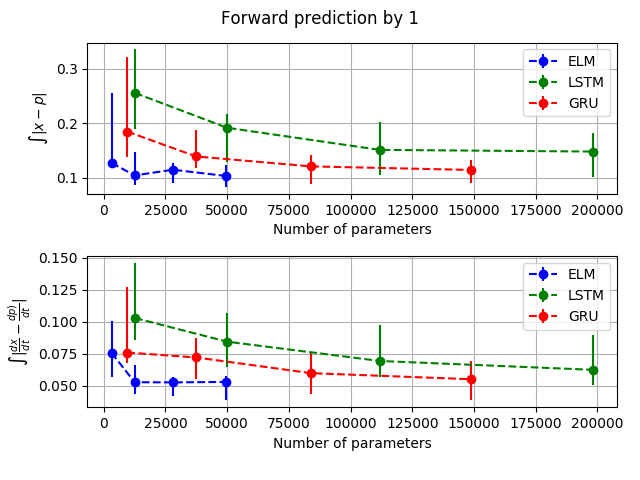
\includegraphics[width=\textwidth]{figures/mg2_scatter_1.png}
     \caption{}
   \end{subfigure}
   \begin{subfigure}{.48\textwidth}
     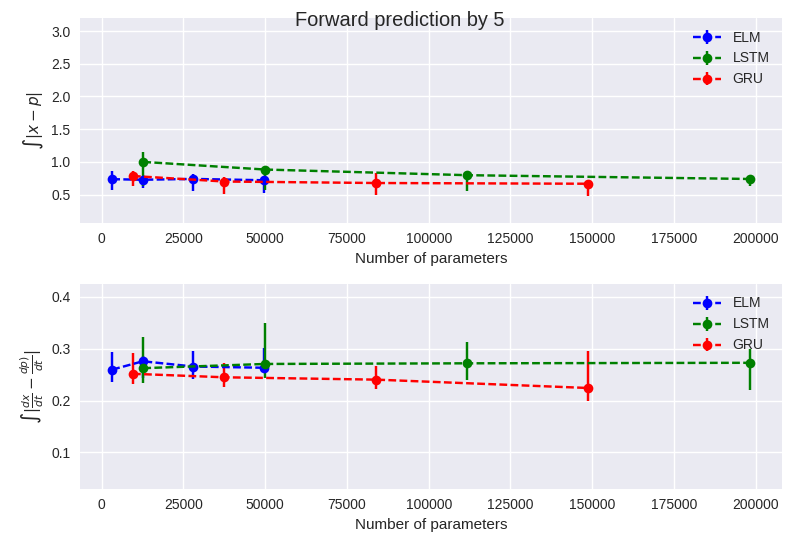
\includegraphics[width=\textwidth]{figures/mg2_scatter_5.png}
     \caption{}
   \end{subfigure}
   \begin{subfigure}{.48\textwidth}
     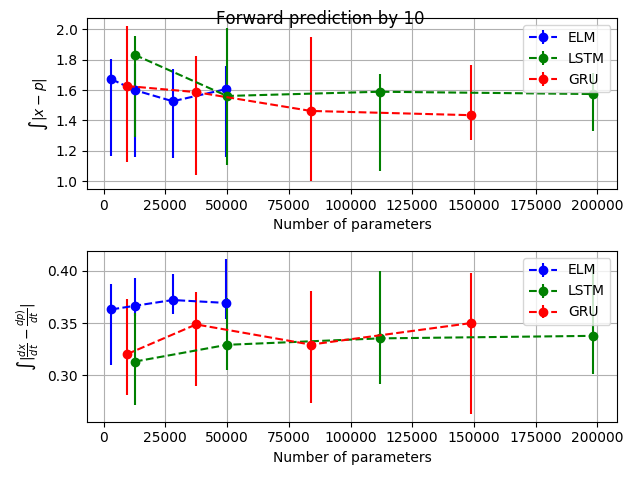
\includegraphics[width=\textwidth]{figures/mg2_scatter_10.png}
     \caption{}
   \end{subfigure}
   \begin{subfigure}{.48\textwidth}
     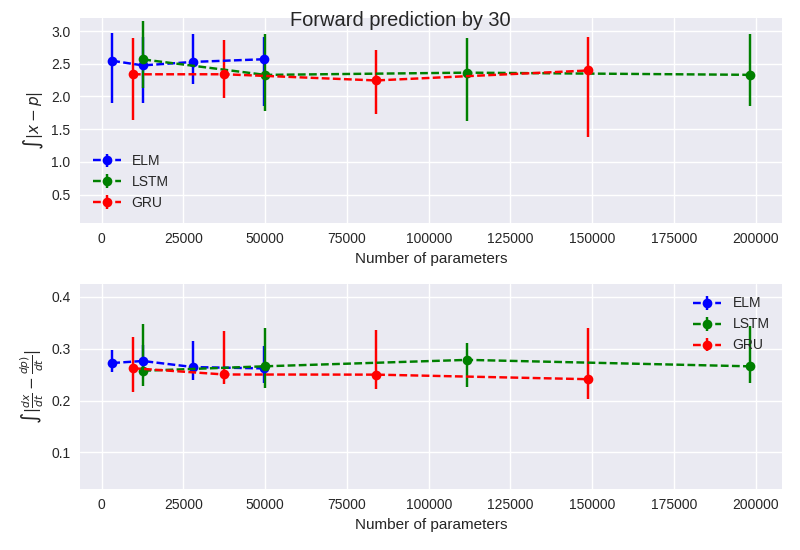
\includegraphics[width=\textwidth]{figures/mg2_scatter_30.png}
     \caption{}
   \end{subfigure}
       
    \caption{Scatter plots showing model performance with different
      network configurations in experiment 2. Leave-one-out evaluation with 10 different MG series was used to generate the data points. All other conventions are the same as Figure \ref{fig:mg1_scatter}.}
    \label{fig:mg2_scatter}
    \end{center}
  \end{figure}

  \begin{figure}
    \begin{center}
   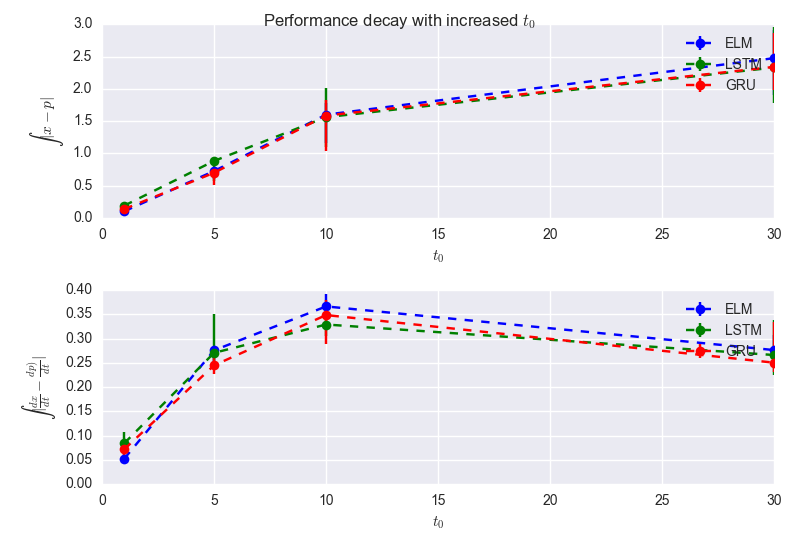
\includegraphics[width=.96\textwidth]{figures/mg2_save.png}      
    \caption{Scatter plot showing the performance of models  as they are trained to predict values further
      in time with a randomized $\beta$.}
    \label{fig:mg2_save}
    \end{center}
  \end{figure}

\section {Discussion}
It should be quite clear that the gated recurrent networks did not have
an advantage over the non-gated Elman network for this predictive
forecasting task. This could be because the ability to recall specific 
information between time steps is less useful for this task, since the
MLP showed a non-linear approximation can work despite $\tau$ being
different from the control points. As the LSTM was designed for tasks requiring distant recollection
\cite{LSTM}, this could explain why the LSTM has such better
performance in tasks like natural language processing, but fails to make a difference in this
instance of predictive forecasting. Although the number of models
evaluated (10) was too small to test with parametric statistics, there
does not seem to be a consistent difference between LSTM and GRU performance.

In terms of the limitations of this paper, it did not explore gated
networks with external memory, like the NARX network used in
\cite{Farsa}. It should be noted that \cite{Farsa} achieved results
that were three orders of magnitude better than the ones presented in the static
prediction task experiments. Also, due to
time constraints I was unable to perform experiments with other MG
parameters were randomized. This is unfortunate, as varying $\gamma$
may have shown yielded different effects in the models than varying $\beta$. Furthermore, due to
the style of implementation, the Elman networks did not use peephole
connections or gradient clipping like the LSTM and GRU. Finally, there
was no regularization attempts for any model. Adding regularization, such as dropout, could change model behaviour.

As an aside, the cumulative absolute difference in slopes did not have
much utility for these experiments. They generally followed the same
trend as cumulative absolute difference, and was a less
intuitive measure for how well the prediction fit to the true prediction. %%

For future work, I would like perform a similar analysis with dynamic
MRI time series images.

 \section{Conclusion}
I used the MG series to evaluate the performance of gated-recurrent
networks, the GRU and LSTM, against ELM and MLP networks. I created
two  experiments to test this: training with a MG series with
static parameters, and training with an MG series with its $\beta$
parameter randomized. The static experiment showed that the gated
networks performed no better than non-gated RNNs. Varying $\beta$  showed that the MLP was unable generalize with free
parameters. Also, there much larger reduction in accuracy for
predicting distant values, but nonetheless, there was little
difference between gated and non-gated RNNs within the number
of configurations attempted on a whole.
% \appendices{}
\clearpage
\bibliographystyle{abbrv}
\bibliography{ref}

\clearpage
\section*{Appendix}
 Sample evaluations for experiment 1 are presented
  in Figure \ref{fig:func_evals}.  Note how the cumulative
   differences begin large and increase constantly throughout the
   evaluation. The inital error is likely due to the hidden nodes
   being uninitialized.

Figure \ref{fig:mg2_func} shows sample evaluations for training with a
free parameter $\beta$. In this
case the cumulative metrics seem to spike periodically in sync
with the peaks of the MG function. This seems to suggest that the
models have greater difficulty predicting large change in slopes than
in the previous experiment, with the predicted spikes occurring before
or after the actual point. %Move this bit to harder predictions

 \begin{figure}[t]
   \begin{center}
    \begin{subfigure}{0.48\textwidth}
      % 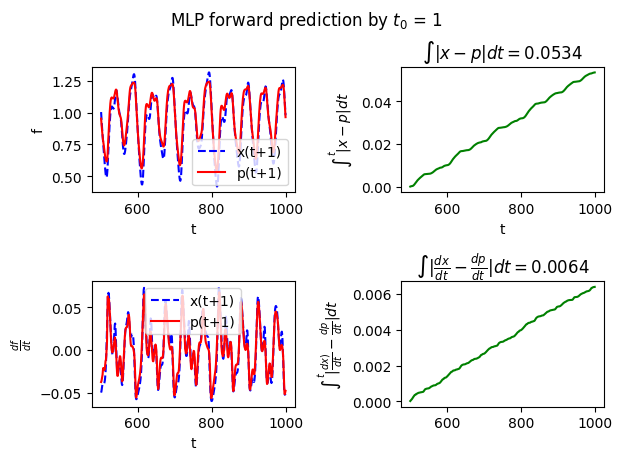
\includegraphics[width=.48\textwidth]{figures/MLP_1.png}
      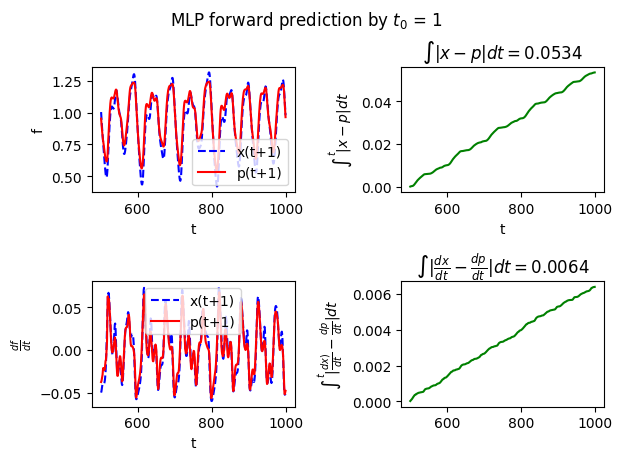
\includegraphics[width=\textwidth]{figures/MLP_1.png}
      \caption{}
      \label{fig:mg2_func_MLP}
    \end{subfigure}
    \begin{subfigure}{0.48\textwidth}
      % 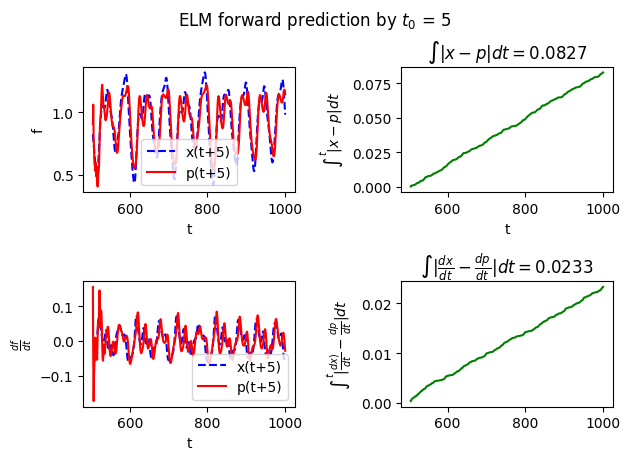
\includegraphics[width=.48\textwidth]{figures/ELM_5.png}
      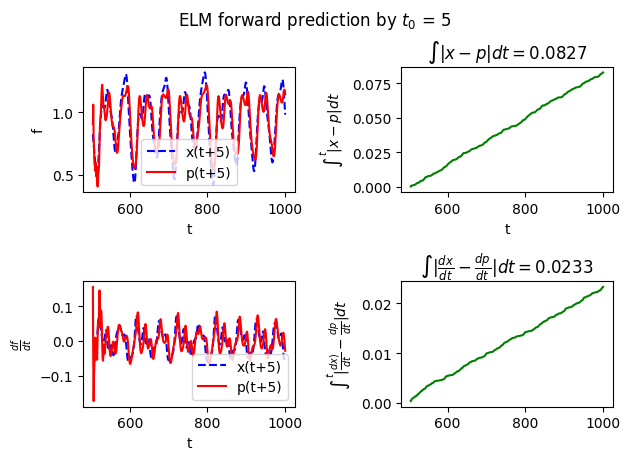
\includegraphics[width=\textwidth]{figures/ELM_5.png}
      \caption{}
    \end{subfigure}
      \begin{subfigure}{0.48\textwidth}
        % 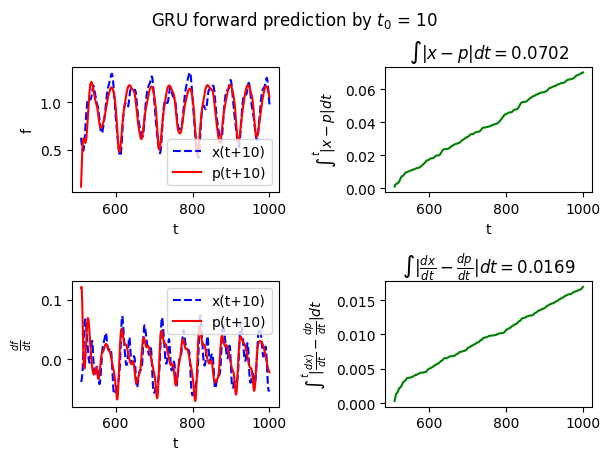
\includegraphics[width=.48\textwidth]{figures/GRU_10.png}
        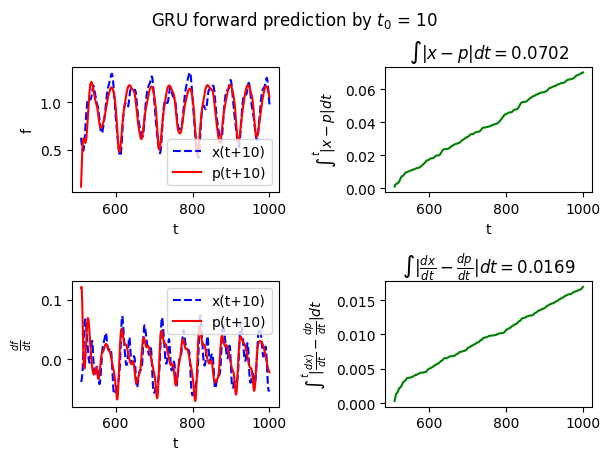
\includegraphics[width=\textwidth]{figures/GRU_10.png}
        \caption{}
      \end{subfigure}
      \begin{subfigure}{0.48\textwidth}
        %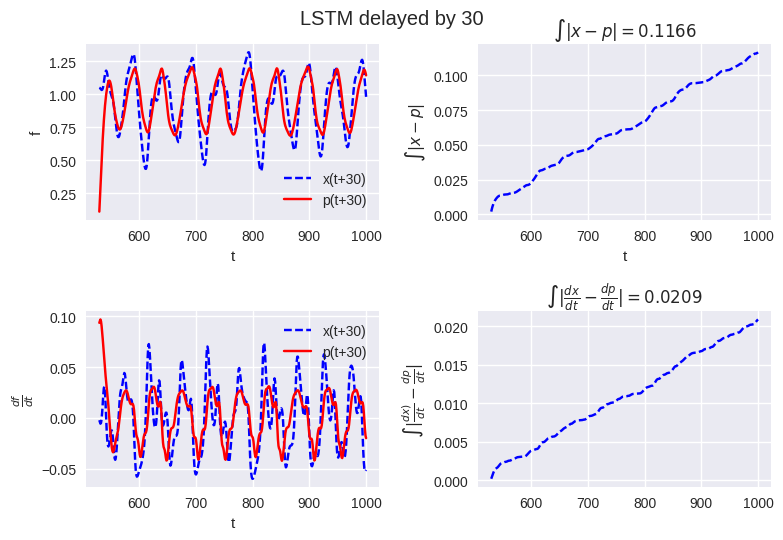
\includegraphics[width=.48\textwidth]{figures/LSTM_30.png}
        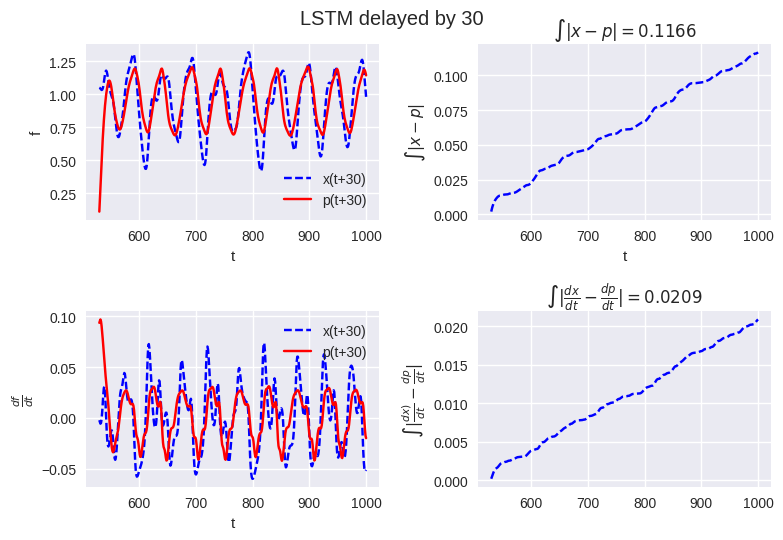
\includegraphics[width=\textwidth]{figures/LSTM_30.png}
        \caption{}
      \end{subfigure}
 \end{center}
 \caption{Sample curve fittings for MLP, ELM, GRU, and LSTM with
   delays of 1, 5, 10, and 30 respectively for experiment 1. The predicted and true
   values of the functions and slopes are plotted, along with the
   cumulative absolute differences metrics.}
 \label{fig:func_evals}
\end{figure}


 \begin{figure}[t]
   \begin{center}
      \begin{subfigure}{0.48\textwidth}
   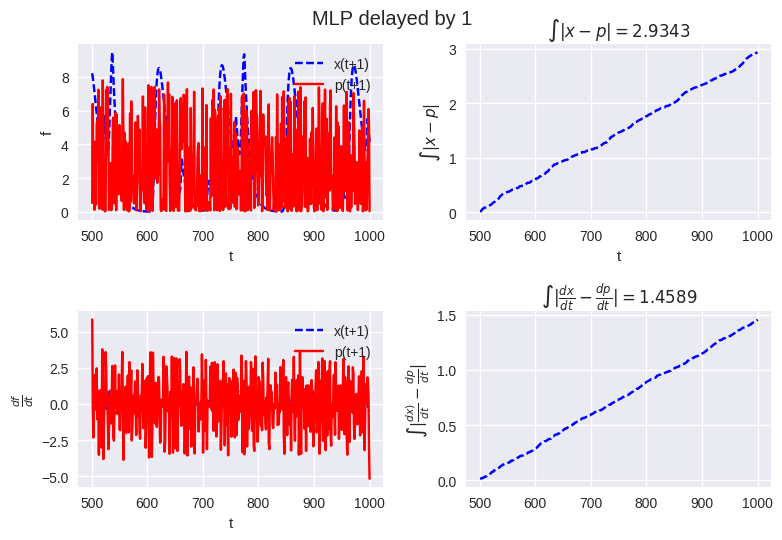
\includegraphics[width=.48\textwidth]{figures/MLP_1_mg2.png}
 \caption{}
      \end{subfigure}
      \begin{subfigure}{0.48\textwidth}
   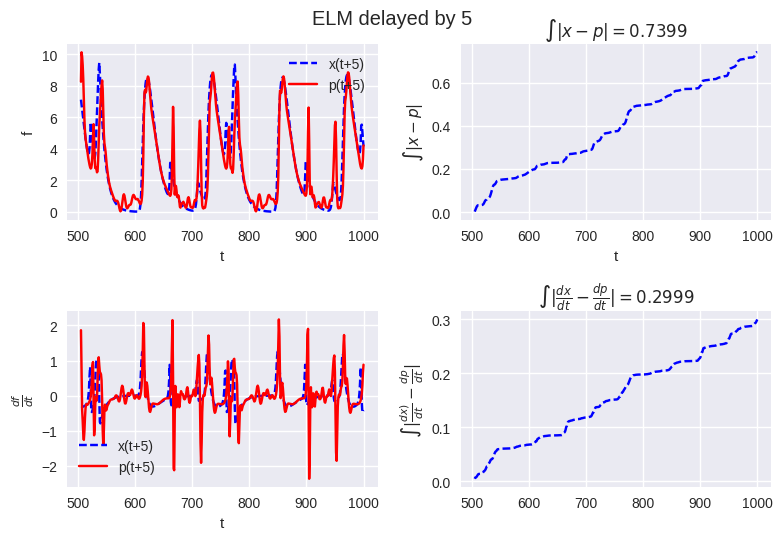
\includegraphics[width=.48\textwidth]{figures/ELM_5_mg2.png}
 \caption{}
      \end{subfigure}
      \begin{subfigure}{0.48\textwidth}
   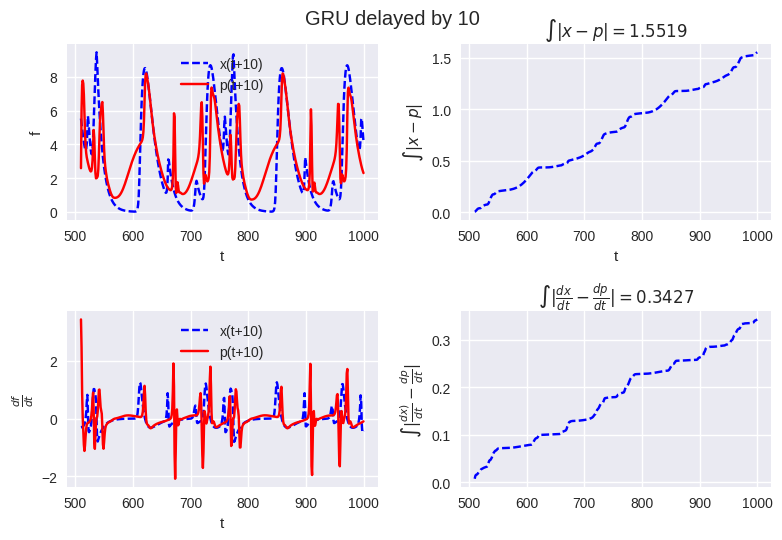
\includegraphics[width=.48\textwidth]{figures/GRU_10_mg2.png}
 \caption{}
      \end{subfigure}
      \begin{subfigure}{0.48\textwidth}
   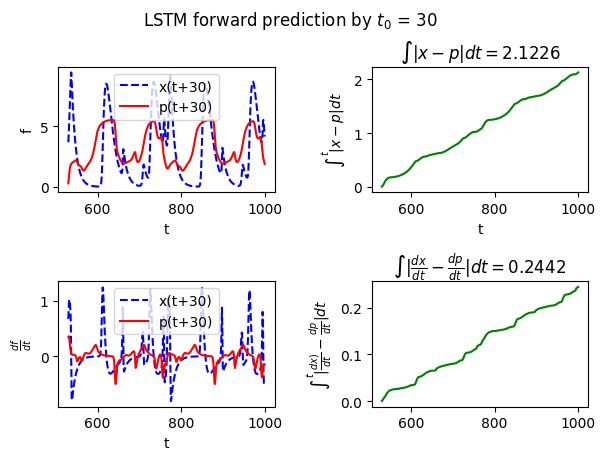
\includegraphics[width=.48\textwidth]{figures/LSTM_30_mg2.png}
 \caption{}
      \end{subfigure}
 \end{center}
 \caption{Sample Curve fittings for MLP, ELM, GRU, and LSTM with
   delays of 1, 5, 10, and 30 respectively for experiment 2. The predicted and true
   values of the functions and slopes are plotted, along with the
   cumulative absolute difference metrics.}
 \label{fig:mg2_func}
   \end{figure}

\end{document}

%Best of beta, 1
% [[             nan   9.99986443e-01   8.55969466e-01]
%  [  1.35570290e-05              nan   1.37114974e-03]
%  [  1.44030534e-01   9.98628850e-01              nan]]
% [[        nan  0.00231888  0.31573538]
%  [ 0.00231888         nan  0.01507229]
%  [ 0.31573538  0.01507229         nan]]

% 5
%  [[        nan  0.98129891  0.00193322]
%  [ 0.01870109         nan  0.00193328]
%  [ 0.99806678  0.99806672         nan]]
% [[        nan  0.06711848  0.01791756]
%  [ 0.06711848         nan  0.01791788]
%  [ 0.01791756  0.01791788         nan]]

%  10
%  [[        nan  0.71123879  0.18053602]
%  [ 0.28876121         nan  0.08266376]
%  [ 0.81946398  0.91733624         nan]]
% [[        nan  0.59110278  0.38488576]
%  [ 0.59110278         nan  0.19871669]
%  [ 0.38488576  0.19871669         nan]]

% 30
%  [[        nan  0.02597448  0.00566875]
%  [ 0.97402552         nan  0.09943508]
%  [ 0.99433125  0.90056492         nan]]
% [[        nan  0.08382948  0.03212341]
%  [ 0.08382948         nan  0.23094991]
%  [ 0.03212341  0.23094991         nan]]
